
\begin{figure}[H]
\centering 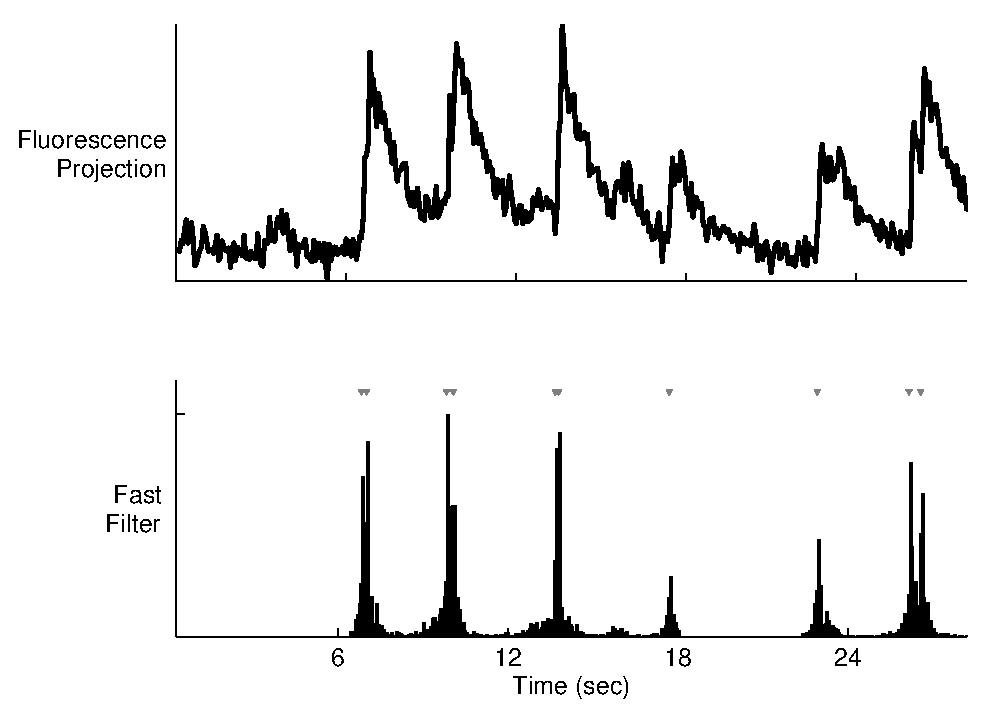
\includegraphics[width=.9\linewidth]{../figs/spatial_data}
\caption{Given only a fluorescence movie, recorded in vivo, we can learn the parameters necessary to correctly infer the spike trains. Top left: mean frame.  Middle left: projection of movie onto mean frame. Bottom left: the fast filter's inference using the mean frame as the filter ($\lam$ and $\sig$ estimated as described by equations \eqref{??} and \eqref{??}, respectively).  Right panels: same as left, but estimating $\balpha$ and $\bbeta$ as described in text.} \label{fig:spatial_data}
\end{figure}

\begin{figure}[H]
%\centering 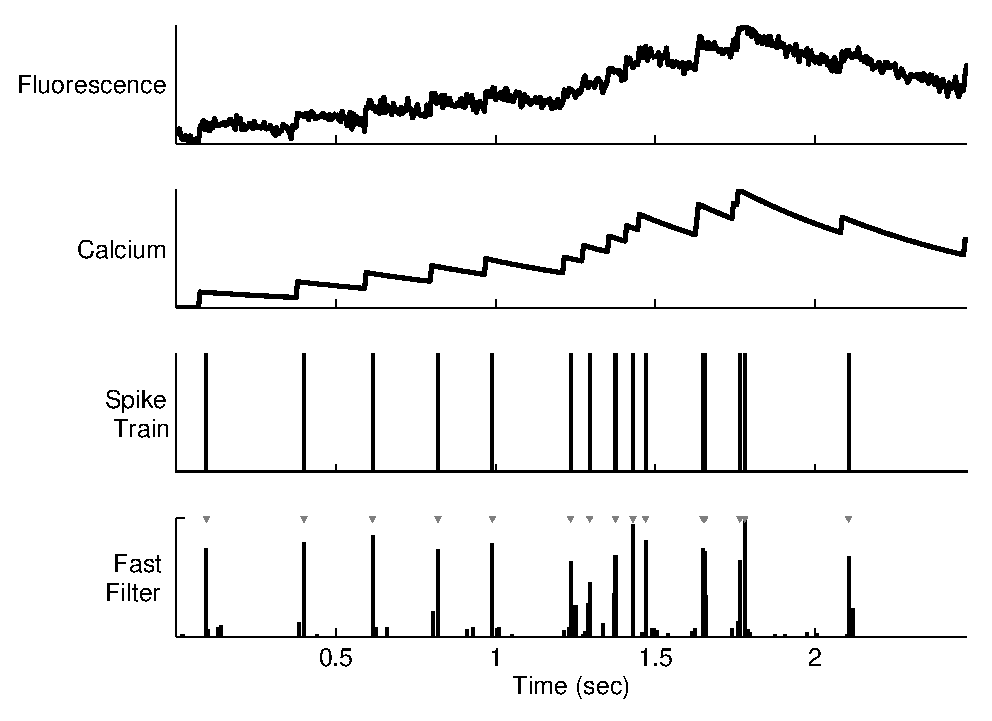
\includegraphics[width=.9\linewidth]{schem}
\caption{distribution of errors in spike inference from real data} \label{fig:err}
\end{figure}


